\documentclass{article}
\usepackage[minionint,mathlf,textlf]{MinionPro} % To gussy up a bit
\usepackage[margin=1in]{geometry}
\usepackage{graphicx} % For .eps inclusion
%\usepackage{indentfirst} % Controls indentation
\usepackage[compact]{titlesec} % For regulating spacing before section titles
\usepackage{adjustbox} % For vertically-aligned side-by-side minipages
\usepackage{array, mathrsfs, mathrsfs, mhchem, amsmath} % For centering of tabulars with text-wrapping columns
\usepackage{hyperref, chemfig}
\usepackage{subfigure}
\usepackage[autolinebreaks,framed,numbered]{mcode}
\newcommand{\Lapl}{\mathscr{L}}

\pagenumbering{gobble} 
\setlength\parindent{0 cm}
\begin{document}
\large

\section*{Introduction to amorphous computing}

Function coordinated through many unreliable parts.

\section*{The Kilobot}

The specifics of the ``hardware" are unimportant, in principle, since amorphous computing is chiefly concerned with describing fault-tolerant algorithms. However, since many studies to date make use of robotics rather than biological systems as a proof of principle, it is worthwhile to demonstrate that we have ``nothing up our sleeve" so to speak -- that is, that all of the features used in those systems could conceivably be implemented in a biological system.

\begin{center}
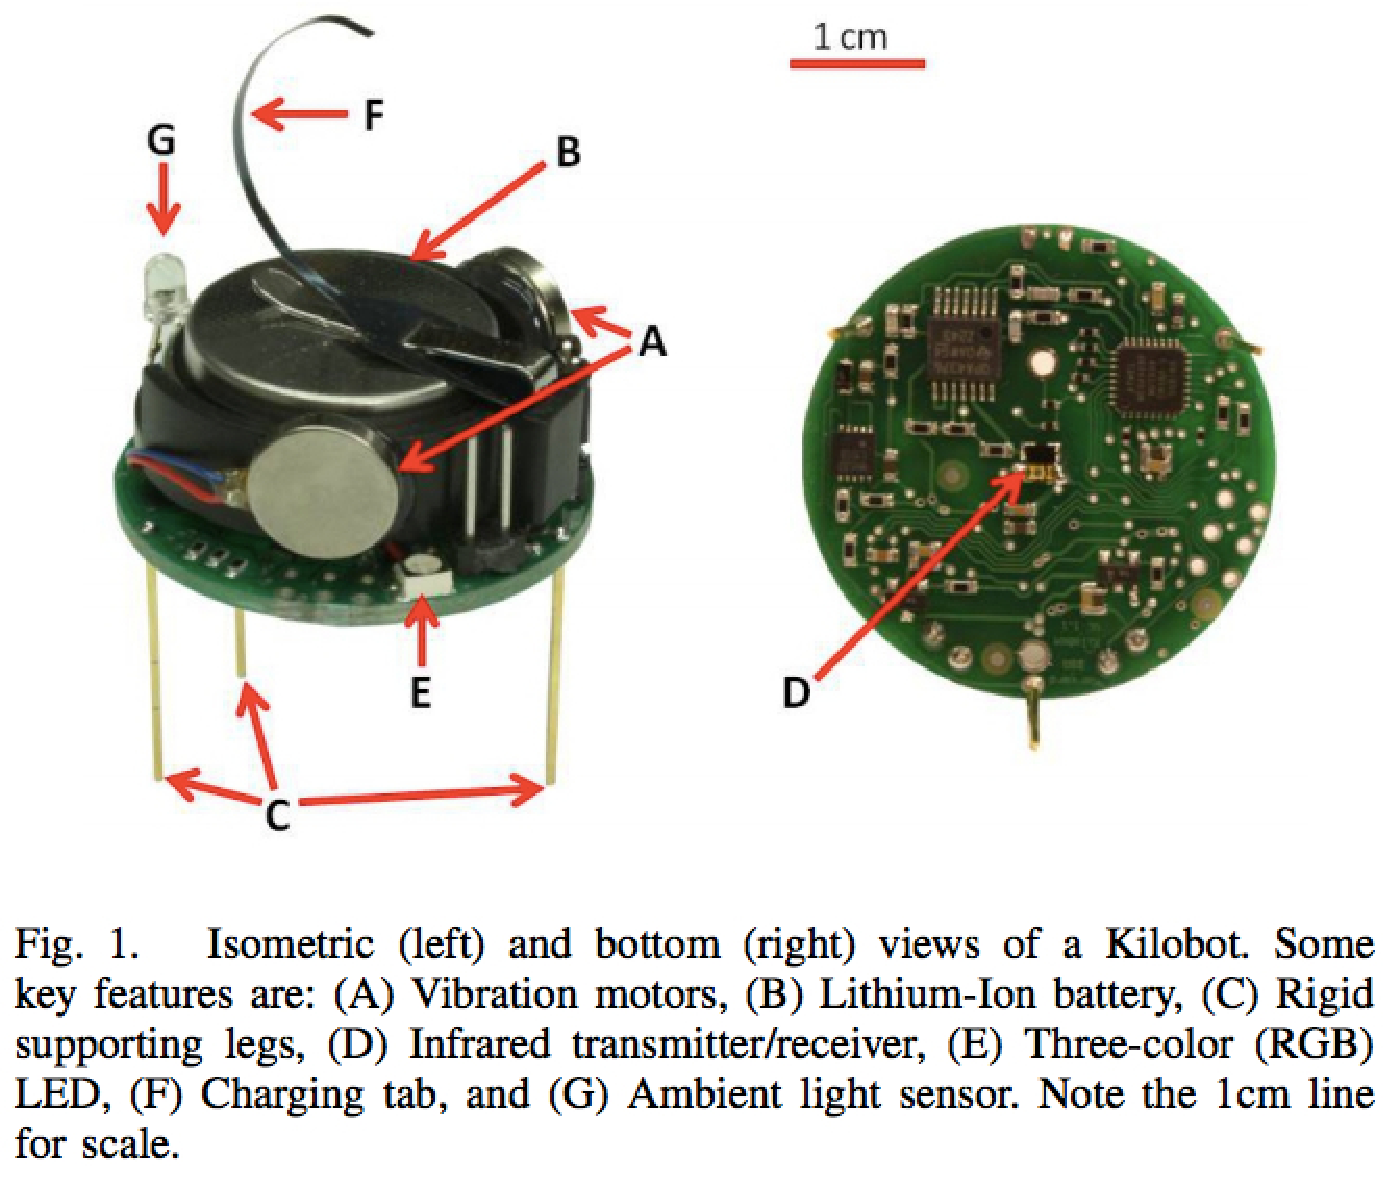
\includegraphics[width=0.5\textwidth]{kilobot.pdf}
\end{center}

The kilobot which will feature prominently in today's lecture: this robot can be constructed in under five minutes for under \$15 (Rubenstein et al., 2012). At this price point, Radhika Nagpal's lab has been able to perform experiments using one thousand kilobots. The robot has no power switch (the designers note that with a swarm this size it would take about an hour to turn them all on) but rather a protruding charging tab. Though its legs are rigid, vibration motors allow the kilobot to move through slip-stick motion at up to 1 cm/s forward or 45 degrees/s rotationally. Precise movement, as with many biological systems, is quite difficult without feedback (but cf. Wittlinger et al., 2006 for a fascinating discussion of odometry in ants).\\

The kilobot can also communicate with neighbors by IR, which it does by reflecting the signal off the surface underneath it (usually, a dry erase board): the angle of reflection limits the distance over which it can communicate to about 10 cm (6 robot widths). Its internal state can be visualized with a color LED. It also has a gratuitous ambient light sensor. All of these features have biological correlates.

\section*{Scaling and shape formation}

SDASH is an algorithm for reliably forming a pattern even if the number of units within a collective is not known or is changing. The only assumptions are that units can determine their position on the plane, which can be done by communication with nearest neighbors and some sort of fixed beacon representing the origin. The collective first attempts to determine its own size through communication with its neighbors. Each unit determines how many neighbors it can contact and how many neighbors each of its neighbors can contact to find the average number of neighbors in its vicinity. In a second round this value is averaged among all neighbors, etc., allowing information about local density to propagate outward through the collective.\\

The shape is scaled by this consensus guess and units begin to enter the region of the shape in such a way that they do not block the entry of other units, and so that the last spot to be filled will be known to all units. If the last spot to be filled is still empty after the last unit is placed, then there are too few units to complete the shape and its scale must be reduced. Units forced to move by the change in scale return to fill these gaps. If, however, there are units left over after the shape has been completed, they add themselves to the exterior of the shape to expand its scaling. (Detection of whether the ``last spot to be filled" is occupied is performed by neighboring units.)

\begin{center}
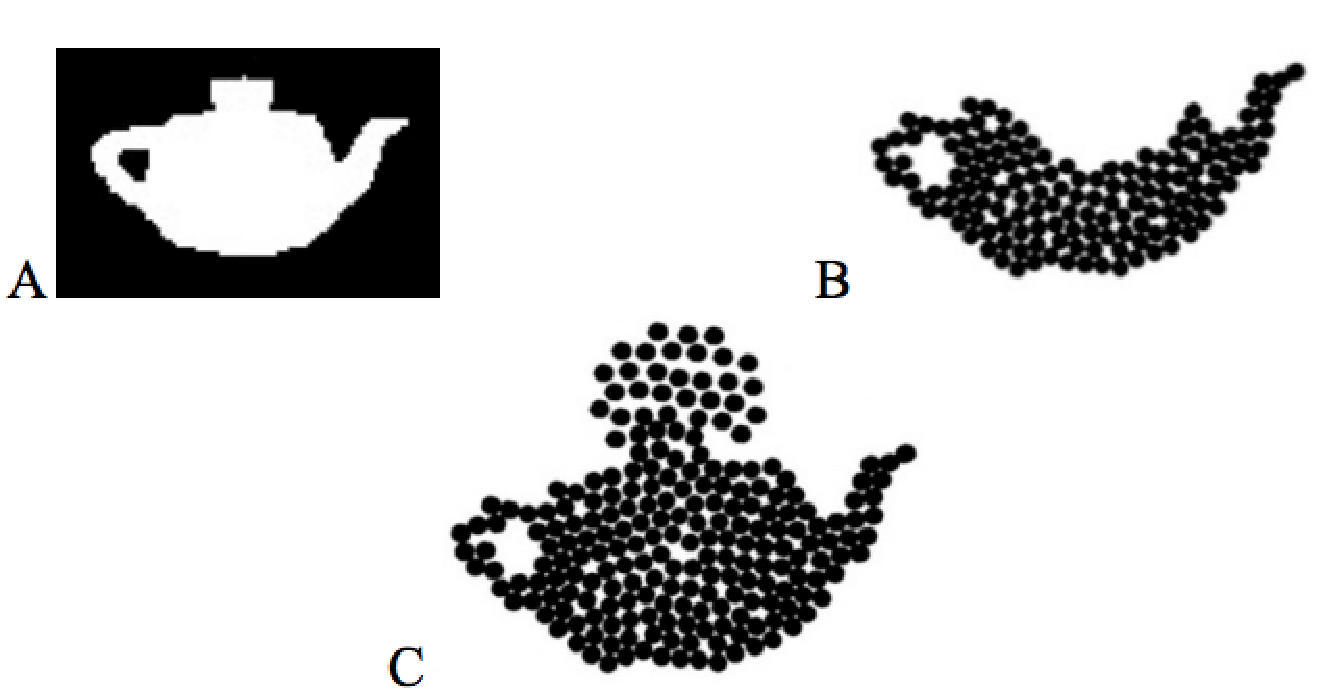
\includegraphics[width=0.5\textwidth]{sdash_errors.pdf}
\end{center}

When units are removed from a completed structure, their neighbors sense the vacancies and regroup to form a smaller structure.

\begin{center}
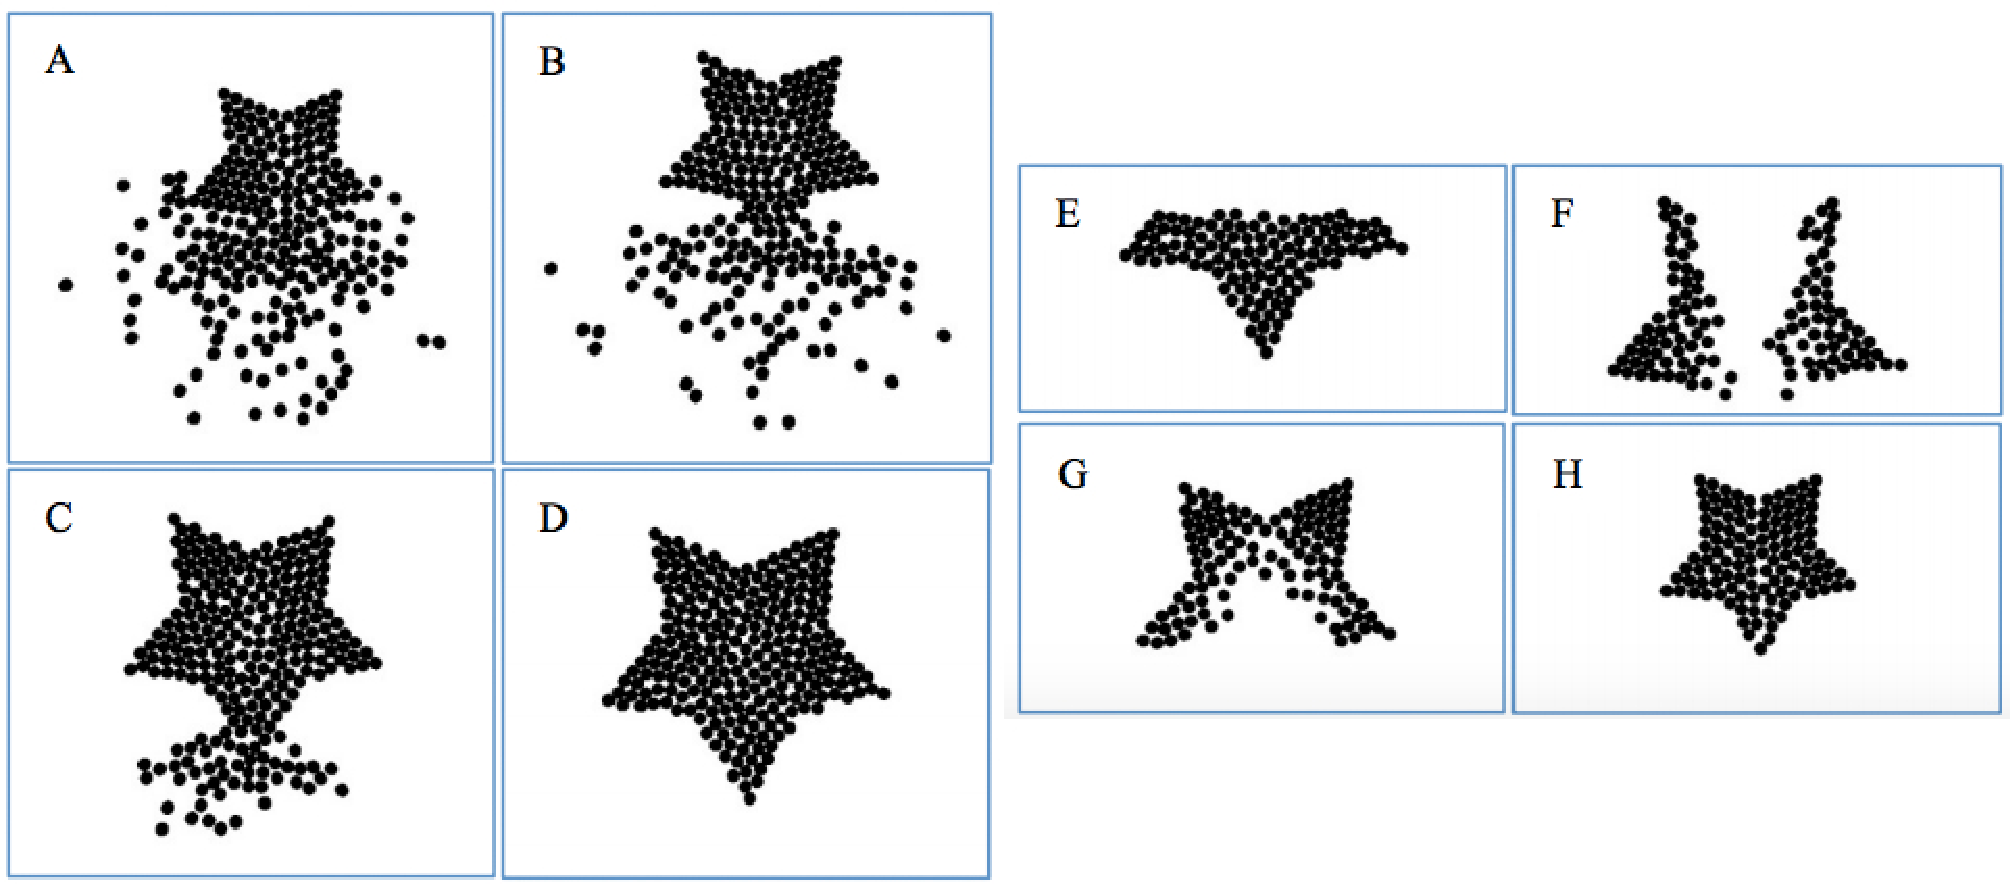
\includegraphics[width=0.5\textwidth]{sdash_healing.pdf}
\end{center}

\section*{Communication}

How do units in a collective share a message across the entire field if their range is limited? A sender that initially broadcasts a message is heard by a few neighbors. To reach a larger audience, we might like to have these neighbors re-broadcast the message. However, if we implement the simple rule that all received messages should be rebroadcasted, then messages will circulate around indefinitely. A simple rule to prevent this propagation is that each message should include a ``hop count": the number of times the message has been rebroadcast so far. The first time a recipient hears a message, it rebroadcasts it and records the hop count for that message. If the same message is then received with a higher hopcount, it is not resent. The same basic principle underlies packet radio networks. Another major issue is that multiple units may try to communicate in the same ``airspace" at the same time, requiring methods for collision detection and resolution (a problem which is made more complicated by the fact that recipients may detect collisions even when neither sender can).

\section*{Swarming}

\section*{Formation of groups}

Suppose we have a field full of identical units that we would like to spontaneously assemble into smaller groups, which might cooperate to perform some function. One simple method to achieve this requires some individuals to identify as leaders and then to force the subservience of those around them. For example, each unit might initiate a timer to a random number: if the timer reaches zero before the unit has heard anything, it will declare itself the leader to all units within earshot. Rare conflicts between leaders can be resolved in a second step. Many units will become members of multiple groups. Once the group has been defined, the ``leader" must retain its specialized function, since it is possible that the leader is the only group member that can communicate directly with all others. This poses a problem, because if the leader unit should malfunction then the group may become non-functional.

\begin{center}
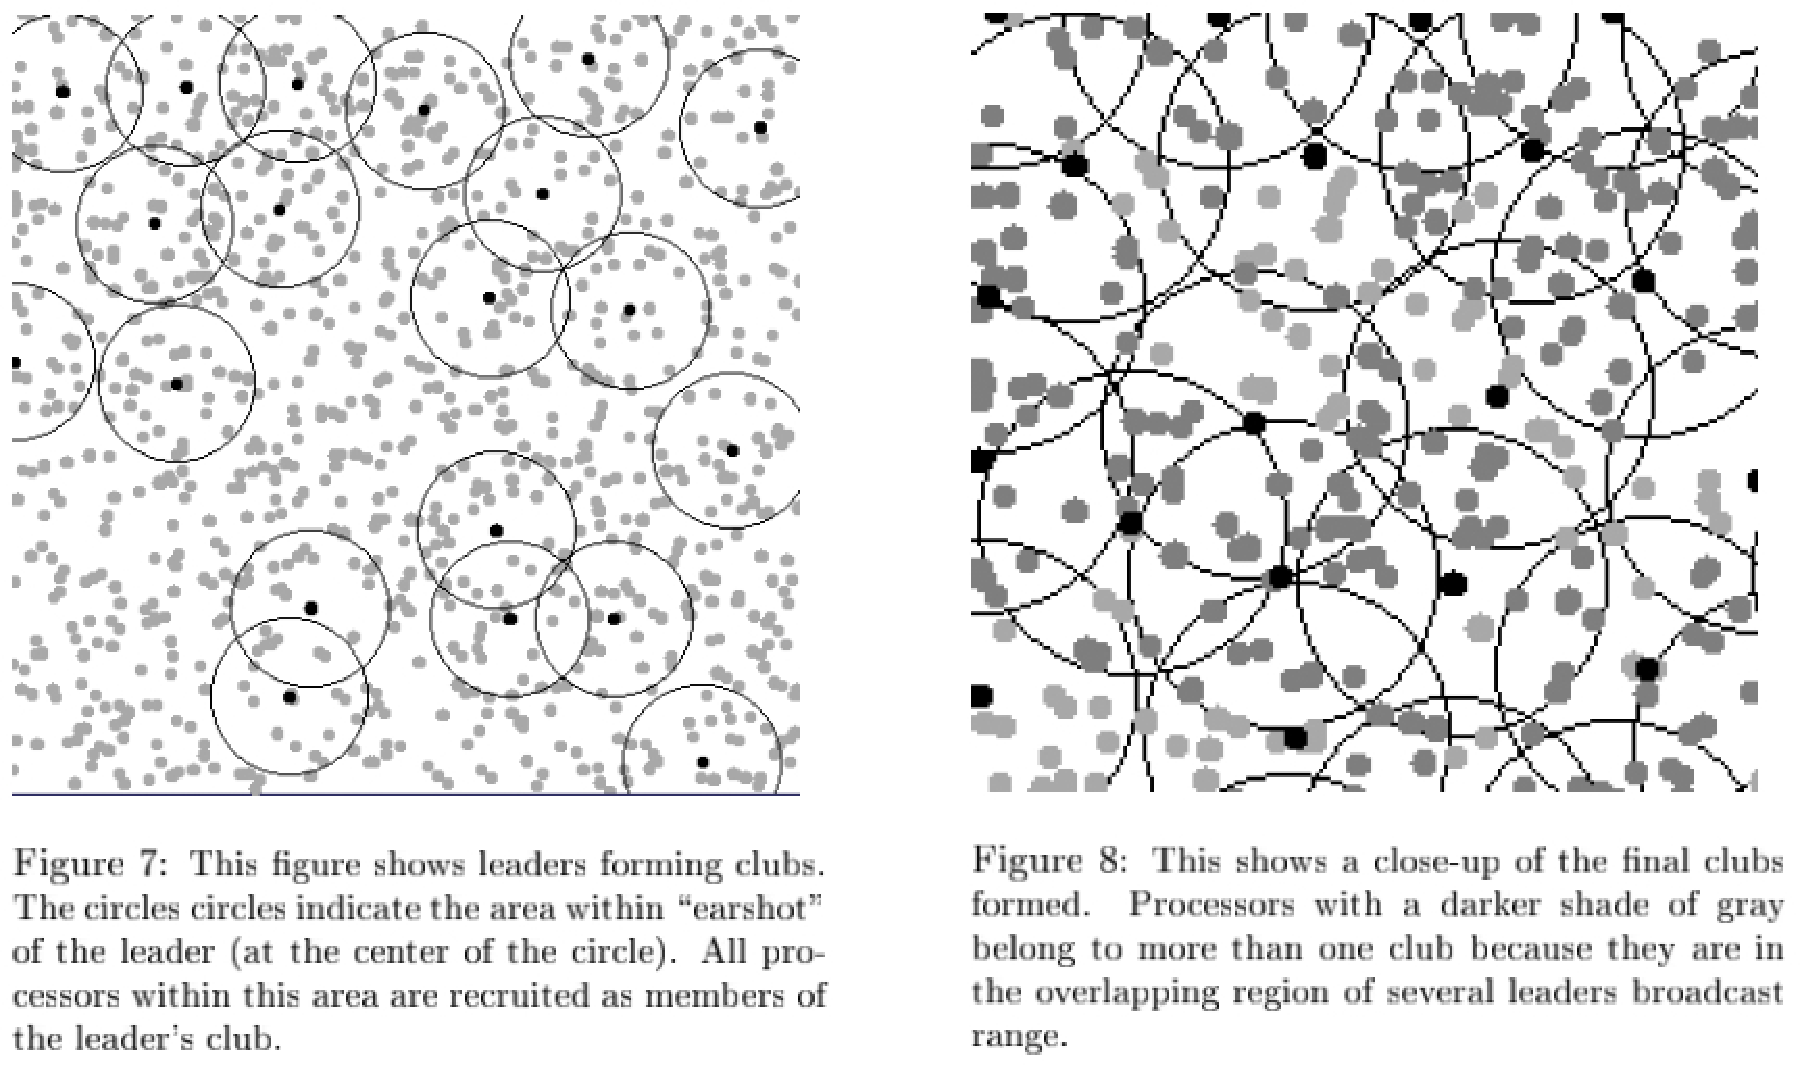
\includegraphics[width=0.5\textwidth]{overlapping.pdf}
\end{center}


An alternative that does not require a permanent leader assumes that each unit has a locally-unique numerical identifier. Each unit determines whether it has the lowest numerical identifier of all units within its communication range: if so, it becomes a ``recruiter" that attempts to bring nearby units into its group. A unit is added if and only if every existing member of the group is able to communicate directly with that unit. While this process requires more querying, it ensures that the resulting group will be able to communicate among itself no matter which units might malfunction later (Coore et al., 1997).


\subsection*{Cheaters}

One recognized issue with the formation of cooperating groups of organisms is that members which are disposed not to cooperate can take advantage of those who are. For example, non-cooperators might use more than their fair share of resources within any group. One way of avoiding interactions with cheaters (assuming that cheating is genetic and mutations that cause it are sufficiently rare) is to form groups only with genetically related organisms. Sometimes a mechanism for interacting only with closely-related units is obvious: for example, many multicellular organism are formed through the sustained interactions of cells descendant from a recent common ancestor. It is less clear whether and how organisms within communities reckon degree of relatedness (or come to count upon it based on typical circumstances): the evolution of altruism remains only partially explained.\\

J. Maynard Smith showed that even if non-cooperators increase in frequency within each group, they can decrease in frequency within the population at large, using a beautiful analogy of field mice overwintering in haystacks (1964). Cooperators can prevail at the population level if the rate of group growth increases with the initial fraction of cooperators\footnote{A striking everyday example of this phenomenon, sometimes called Simpson's paradox, is a lawsuit filed against UC Berkeley in the seventies for discrimination against women after grad school admissions data revealed that 44\% of male applicants were admitted vs. 35\% of female applicants. It transpired that in almost every department, a higher percentage of female applicants were admitted than males; however, women were more likely to have applied to departments where the competition for admission was stiff (e.g. English) than were men.}. More recently Stan Leibler's lab at Rockefeller has confirmed this effect experimentally using bacterial cultures (Chuang et al., 2009).

\begin{center}
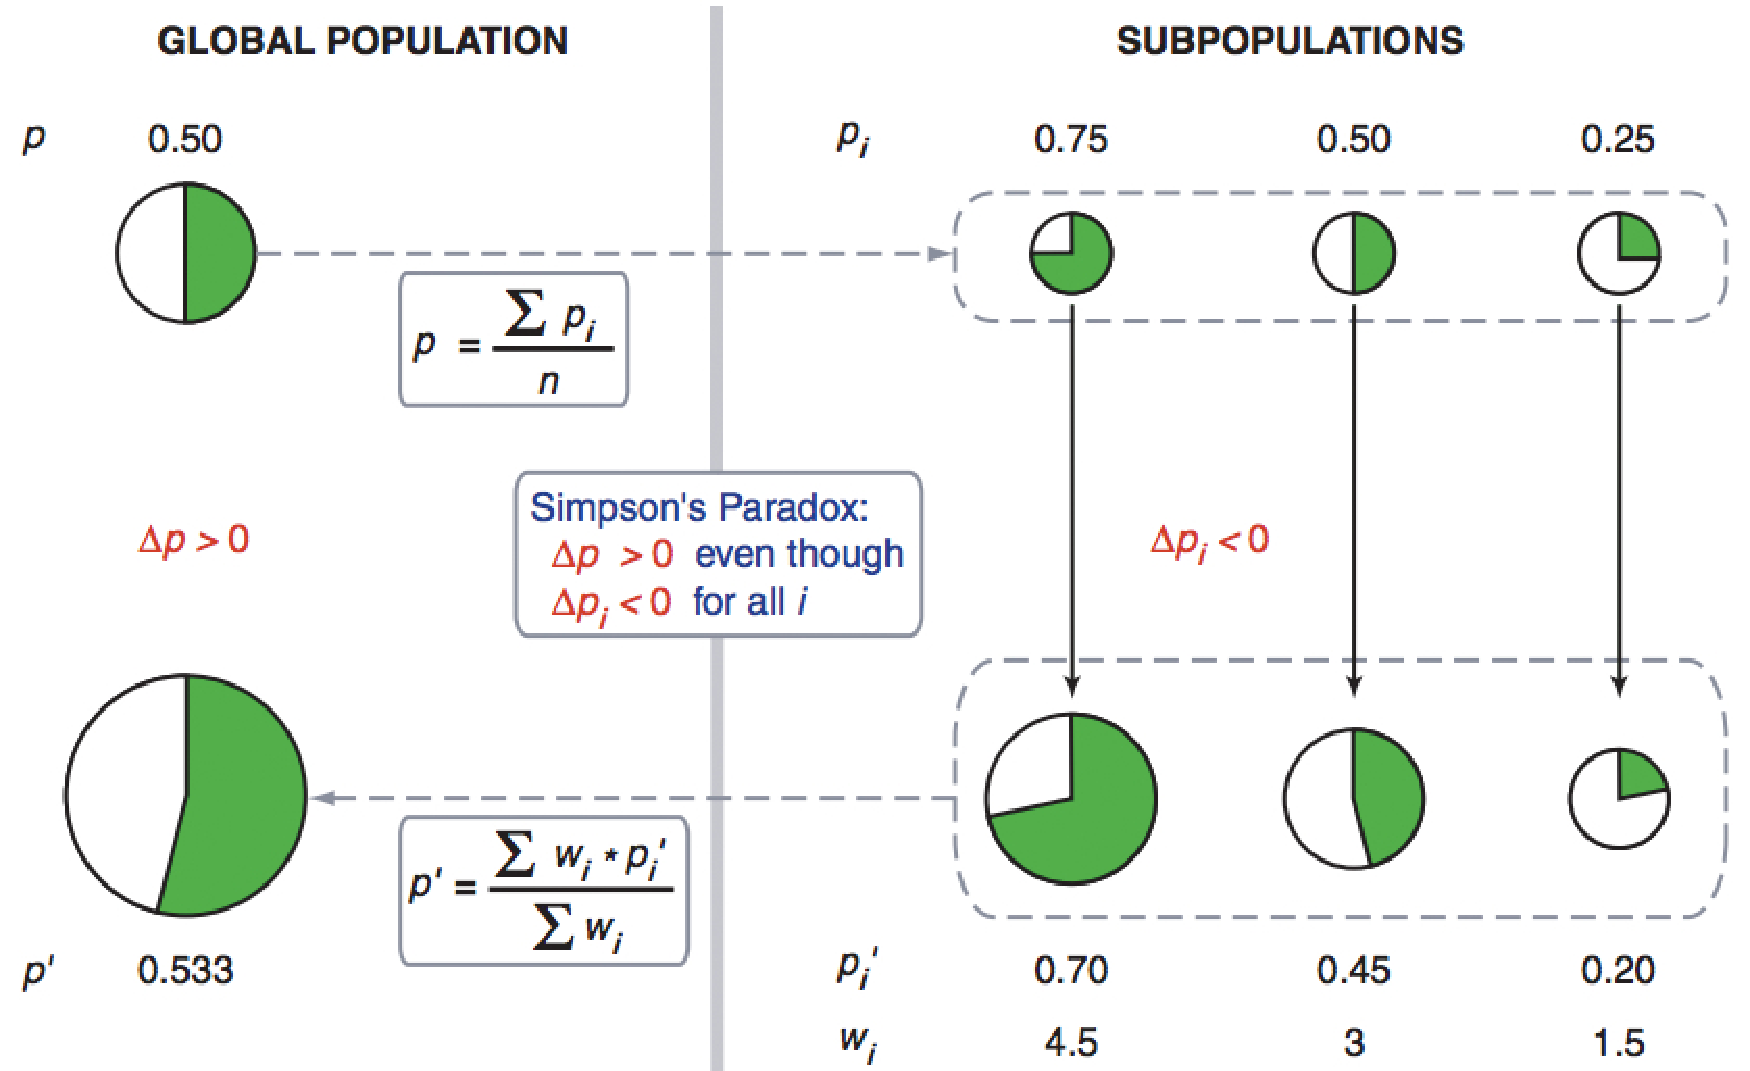
\includegraphics[width=0.7\textwidth]{chuang_fig.pdf}
\end{center}


\end{document}